\documentclass{article}
\usepackage[utf8]{inputenc}
\usepackage[T1]{fontenc}
\usepackage{graphicx}
\usepackage{hyperref}
\usepackage{geometry}
\geometry{margin=1in}

\title{Britannica Volume 144850377 Row 1904}
\date{Encyclopaedia Britannica (1771)}

\begin{document}
\maketitle

\section*{Historical source}
\textbf{Entry ID:} \texttt{entry-britannica-volume-144850377-row-1904-1904} \\
\textbf{Volume ID:} 144850377 \\
\textbf{Character Count:} 12243

\subsection*{Extracted Text}
**LY R [ 4329 ]** **L Y R**

Lyre, which he ufd to frequent, at the foot of a mountain in Arcadill. In all as he was going in, he found a tor- tulofe finding at the entrance of his case: he killed him poor creature, and perhaps, vat the flesh of it. As he was diverting himself with the flesh, he was migliedly pleafed with the molle of great from his concave figure. He had puffily been cunning enough to find one, that a thong pulled fruit and affected is each end, when freds by things you take aird mudiculous. How ever that was, he went immediately to work, and eut feveral things out of the links he had lately flolen, and afected them as right as we could on the field of the tortofie and, in playing with them, made a new kind of mute with them to divert himself in his retreat. This, considered only as an account of the first inven- tion of the lyre, is not altogether for unsurals?

The most ancient representations of this instrument ages very well with the account of its uncertain the lyre, in particular on the old echelith globes, was re- prefered as made of one entire shell of a tortorise; and that, Amphibus in the celebrated group of the Diver, or Toro, in the Fanerle place at Rome, which is of Greek feulpture, and very high authority, is figured in the fine manner. See Plate EXXL fig. 7.

There have, however, been many other claimants to the fewven-firinged lyre. For though Mercury invented the thin instruments in the manner already related, it's fail for afterwards gave it to a position, who are the first that played upon it with method, and made it the con- fiant companion of pretty. According to Moment ac scount of this transfections, in his hymn to Aftervery, it was given by that god to Apollo, as a peace offering and indemnification for the oxen which he had flolen from him:

Tv Phachos Mais’s fun preints the lyre, A A just intended to aproils like it.

A post contains it aproils, and clays. The need information a threshold was). With exact least full the platform readily, and fines. Most seen according to the resulting fringes. Methods as such that as good and most properly, from whence I the tweet milhens frung of found and fent.

Doulton informs us, that Apollo four reporting of the creety with which he had treated Marxas in confidence of their unified control, broke the fringe of the lyre, and by that means put a flop for a time to any further progress in the practice of that new in frumers. "The music (aida by afterwards added to this infrument the firing called my/y Linas, that of \_Ikshary\_) and Orpheus Thanayas, hide finds which are caused \_Update and participate\_ (i).

Again, many ancient and repeticable authors tell

us, that, before the time of Terpandan, the Grecian lyre had only four fingers and; if so may believe Biduan, is remained in alien face 850 years, from the time of Amphio, till Terpander added to it three new fringes, which extended the mulleical feel to a hope, chord, or events, and luppiled the player with two conjoint tetracothis. It was about 150 years after this period, that Pythogorsa is fast to have added an eighth fringe to the lyre, in order to complete the oc- rave, which conflicted of two disjunctiont herchords.

Bochthia gives a different history of the feels, and tells me, that the flyton did no long remains in fact narrow limits as a tetrachold. Chorobus, the fan of Athis, or Arys, king of Lydia, added a fifth firing; Hyguns, a firstly, Terpandera, a favorite and, at large), Erythema of Samoa, an eighth. But all their accounts are irreconcileable with Momars, hymn to Mercury, where the chelys, or reduce, the invention of which he earlier or than god, is fast to have had been fittings. There are many clamans among the musicians of ancient Greece, to the things that were afterwards added to thefly, by which the date, in the time of Alfoxcoras, was extended to two offices. Athamus, more than once, peaks of the nine fingerling inflamments, and Lon OlChoja rtagies and lyrics pace and philosopher, who fitf recited his pieces in the 8zd olympiad, 452 B. C. mentions, in some refer quoted in Dr. David, the ten- firginged lyrs, a prodt that, the third conjoint tetr- chord was added to the scale in his time, which was about 50 years after Pythagoras is fuppelled to have confinational the death.

The different claimants among the Grecks to the famedual differences, only proxy, that made was cul- treated in different countries, and thus the inhabitants of each country invented and improved their own in-fruments, none of which happening to celebrate those of other parts of Greece, resident it difficult for his- florions to avoid attributing the fame invention to dif- ferent periods. Thus the Eagle Rule we give to Mi- nerva, and to Marfayas theynas, or filialty, to Pan, and to Cybele, and the lyre, or citura, to Mercury, Apollo, Amphioa, Lima and Opheus. Indeed, the mere addition of a living or now to an infiltration with on a neck, was fo obvious and early, that it is scarce podible not to conceive many people to have done it at the fame time.

With respect to the form of the ancient lyre; as little agreement is to be found among authors as about the number of things. The belt endurance concerning it are the representations of this inflamment in the hands of ancient flatues, bas-reliefs, etc. See Plate CLXI.

Lightning, we have few always; it is \_mattematically couldn’t\_, that, when a \_returning firele\_ comes to be produced by the \_fuddro\_ removal of the very frong elafic electrical prefi-fore of the electrical atmosphere of a thunder-cloud powerfully charged; the frength of such a retraining \_fireks\_ mult be enormous.

" If indeed the quantity of electric field naturally contained in the body of a man, forrindance, were often mefe, or induding, the author's ultimate between the effects producible by a cloud, and those caned by a prime conductor might be admitted. But fairly electronic cloud,—how great forces may be its extent, and the height of its charge, when compared with the scenes and change of a prime conductor-- cannot cepel from a mared (way (only other key)) more than the natural quantity of electricity which it contains. On the fodder removal, therefore of the preffure by which this natural quantity had been expelled, in consequence of the equation of the cloud into the earth) so more (at the utmost) than his \_robole natural lack\_ of electricity can re-enter the body (c). But we have no reason to fopate that this quantity is fo great, as that its fudden re-entrance into his body found delivery on even injury third " At the experiment above deferbed, the infulated perfor receives into his body, at the infant of the \_returning firele\_ has only all that portion of his own natural electric-free which had been expelled from it; but likewise transmits through it, at the fame infant, \_its consequences of the peculiar fluctuation\_, all the electric fire of which the large cloud could had been robbeds and which mult needeffally re-pafa through his body, to arrive at that conductor. To render the cafe foreshable instability in natural electricity, the man's body mult be fo peculiarly circumdanced, impunding him to be in a hoofu, that the electric matter which has been expelled from the head into the earth, by the preffure of an extensive thundercloud, could not return back into the building, on the explorations of the clouds as different, without paling through his body: a safe not likely to happen, unfuls the boots were in- folated (like the second conductor in the preceding experiments), and his body became the claimed through which where the hole could have the electric matter reflored to it : it appears much more probable that the electric matter returns to the house through the \_fame elements\_ by whole it before recently pafled out, and with equal silence, too more fuddently.

" If the cafe of a man who is abroad, and in an open field, during the time of an explosion —a he is unconnected with other matter of matter above him, no more than the preflic quantity of electric fire, which had been before expelled from his body, will definitely return into it at the infant of a dither explosion; and that this quantity is not uufaly very large, may be inferred from many considerations.

" When a perfon standing on the ground holds a Lightning pair of Mr Canton's balls in his hand, while a highly charged thunder-cloud is fufpended over his head; the angle made by the balla indicates the \_electrical fate\_ of this portion or the quantity of natural electricity of which his body as at the time deprived, by the action of the (\_politively\_) charged cloud hanging over him. But we have never feen the repollion of the balls to fulfillment, as to contain any the apprehensions that the return of his natural electric matter, however fudden, could be attached with his injury to him a nor would be be flexible of any common use the bulk fuddily coming together; the 'a fpark might un-doubtedly be perceived, at that infants, were he infuried, and placed in the four manner with the author when he tried the above-related experiment.

" The author nevertheless observe, that , there have been influences of protons who have been killed by natural electricity, having been found with their \_floos torna\_, and with their feet damaged by the electrical line, but who have not bad, over their whole boo, any other apparent marks of having been ftuck with lightning." He adds, " if a man walking out of doors were to be killed by a returning firele, the electrical line would rub into that each body into his \_feets\_, and his feet only ; which would not be the cafe, here he to be killed by any \_main fireke\_ of exploding, either positive negative.

" It would be no difficult talk, we think, to account for these appearances in different manner, were all the circumstances attending the cage minutely after-tained, but without interrogating the dead on this futjels, we may more falsifiedly appeal to the ex-perience of the living (a), to flew, that though the \_returning fireks\_ mult take place, in all thunder-forms, \_in June degree or other\_; yet it is now of that alarming magnitude within the author afterhes to it. If, a non particular thunder-form, a man in the open fields could be killed, at the infant of a dillank explotion, merely by the returners of his new electric fire, which had before been driven out of his body; lureely numerous obferations of persons who had experienced the \_returning firele\_, in fighting degrees, would be families, and favors a great teacher-theme must have occurred, in which one perform or another mult not, at theinflated an explosion, have felt the effects of the \_returning firele\_, in \_foon degree or other\_ from that of a violent sanctions, to that of a flight and almost impregnible pollution. But no observances we this kind are known to us say how we ever heard of any person's experiencing any kind of electrical com- motion in a thunder-loria, except fish as have either been directly frocks, or have happened to be in the \_royar near neighborhood\_ of the foot where the explodes took place.

" The author has been aware of this objections, which (c) " We fuppie the perfor not to be fo fluuted, that the returning fire of other bodies mult necefarily pafa through his body.

(b) " The author does indeed produce a living evidence, in the cafe of a person at Vienna, who, he has been credibly informed, received an electrical shock, by having held one hand accidentally in contact with an intercepted metallic coaching mind, at the infant that a thunder-cloud exploited at the influence, as was considered, or above half an English milk. He likewise observes, that a very strong, bright, and fulden firek (ce fpars) of electric fire has been been, by levels electrificants, to pais in the internal, or interruption, purposefully left in the concluding rod of a book at the infant do a distant explosions, and ‘when it was fully proved, by the sharp point of the conductor not being melted, or even tuged,' that the conductor itself had not been effect — "Other observations, however, do not by any means prove the magnitude or danger, of the returning broke, but merely its \_esiflessen\_ which we do not contiti."



\section*{Source record}
\begin{itemize}
\item \textbf{Dataset:} \texttt{NationalLibraryOfScotland/encyclopaedia\_britannica\_illustrated}
\item \textbf{Dataset Revision:} \texttt{309f765b1ecc83e0a7f7762e44b4a927a7555443}
\item \textbf{Page ID:} \texttt{britannica:309f765b1ecc83e0a7f7762e44b4a927a7555443:train:1904} \\
  \textbf{Filename:} \texttt{page-1904-759854fd95bb.jpg} \\
  \textbf{Row Index:} 1904 \\
  \textbf{SHA256:} \texttt{759854fd95bb6385...}
\item \textbf{Page ID:} \texttt{britannica:309f765b1ecc83e0a7f7762e44b4a927a7555443:train:1910} \\
  \textbf{Filename:} \texttt{page-1910-f4723acc1771.jpg} \\
  \textbf{Row Index:} 1910 \\
  \textbf{SHA256:} \texttt{f4723acc17718590...}
\end{itemize}

\begin{figure}[h]
\centering
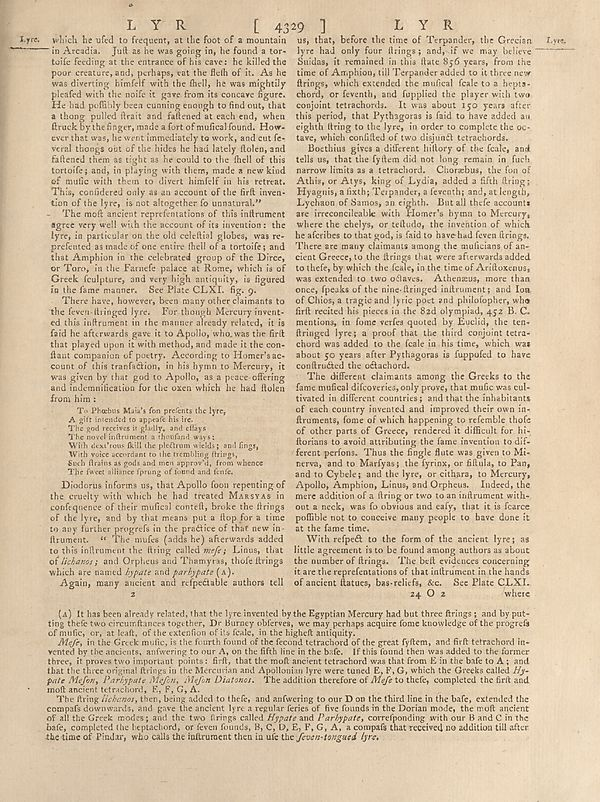
\includegraphics[width=0.85\textwidth]{../scans/page-1904-759854fd95bb.jpg}
\caption*{Source scan: \texttt{page-1904-759854fd95bb.jpg}}
\end{figure}
\begin{figure}[h]
\centering
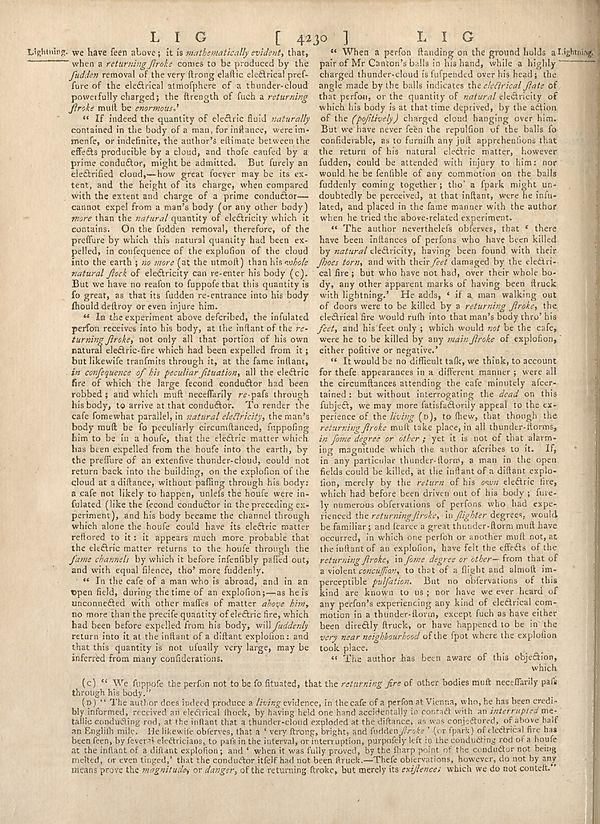
\includegraphics[width=0.85\textwidth]{../scans/page-1910-f4723acc1771.jpg}
\caption*{Source scan: \texttt{page-1910-f4723acc1771.jpg}}
\end{figure}

\end{document}
